\subsection{Introducing CMB temperature anisotropies}\label{sec:CMBAnisotropies}
To study how photons propagate between last scattering surface (LSS) and today consider a flat Universe subject to scalar perturbations (here $\Psi \neq -\Phi$ as we are not working in single perfect fluid approximation), change sign of $\Psi$ for convenience:
\begin{equation}
    ds^2 = a^2(\tau)\left[\left(1+2\Phi\right) - \left(1+2\Psi\right) \delta_{ij} dx^idx^j\right]
\end{equation}
Write down geodesic equation for photons, first with affine parameter $\lambda$, then in conformal time.
\begin{equation}
    \dot{P}^\beta + \Gamma^\beta_{\mu\nu}P^\mu P^\nu = 0 \qquad P^\mu= \frac{dx^\mu}{d \lambda} \qquad \dot{P}^\mu= \frac{dP^\mu}{d \lambda} = \frac{dP^\mu}{d \tau} P^0
\end{equation}
Look at $0$ component and then compute full perturbed connections at first order, in doing so expand $(1+2\phi)^{-1}$:
\begin{equation}
   \frac{dP^0}{d \tau} + \Gamma^0_{\mu\nu}\frac{P^\mu P^\nu}{P^0} = 0 
\end{equation}
Plug the expressions in and use the null condition $P^{\mu}P_{\nu}=0$ to get $P^i = P^0 \left(1+\Phi -\Psi \right) n^i$ 
Where $n^i$ is any unit vector on the sphere (pointing along photon's direction in the comoving spatial frame).
\begin{figure}[h]
      \centering
        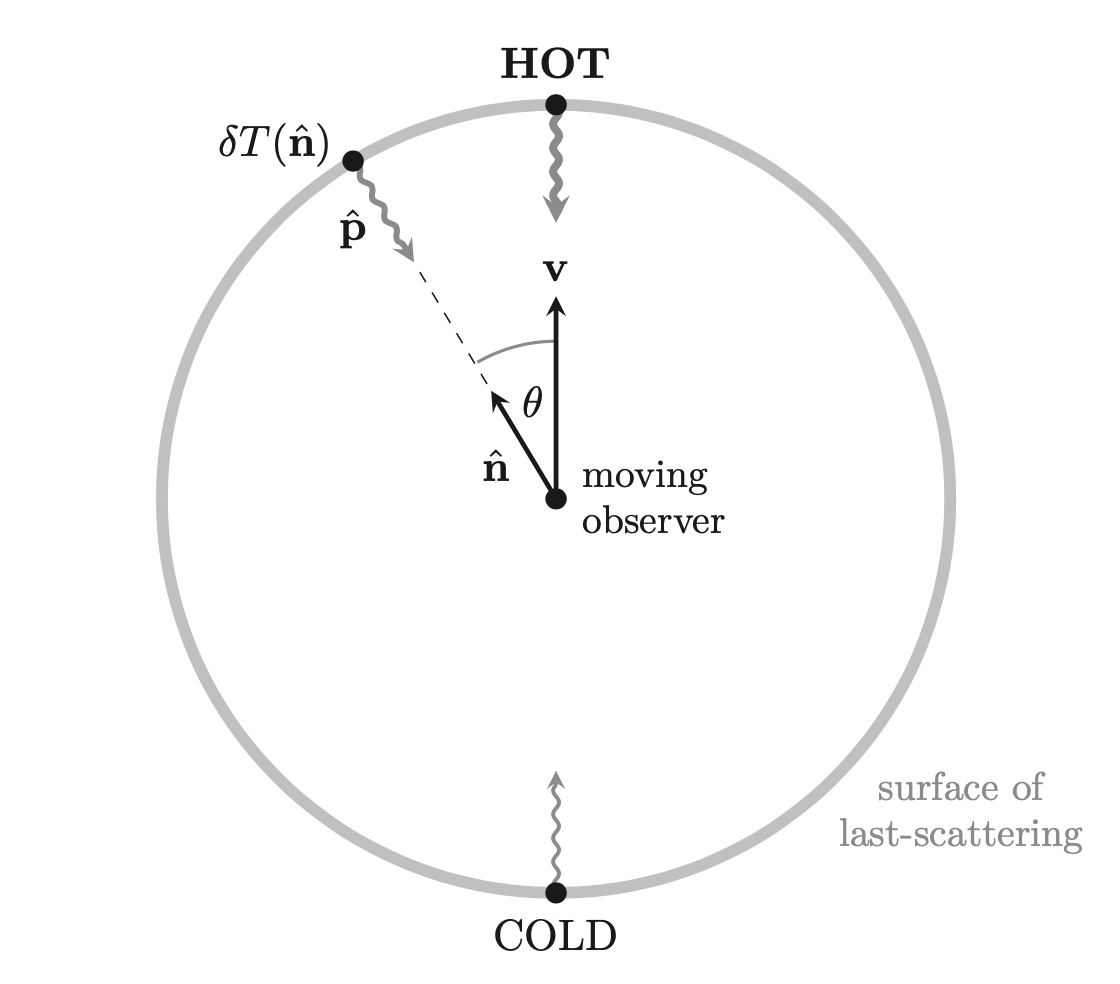
\includegraphics[width=0.8\textwidth]{Graphics/CMB-doppler.png}
        \caption{Motion of the Solar System relative to CMB rest frame~\cite{CosmologyBau}.}
  \end{figure}
This leads to\footnote{Recall $'$ are \emph{partial} derivatives with respect to $\tau$.}
\begin{equation}\label{eq:0thcomponentGeo}
    \frac{dP^0}{d \tau} + 2\frac{a'}{a}P = -P^0 \left(\Psi'+\Phi'\right) -2\Phi_{,i}n^i P^0
\end{equation}
Define the \textit{conformal momenta} \textcolor{darkgreen}{$\varTheta^\mu \equiv  a^2 P^\mu $} to notice that $\varTheta^0$ is conserved at zeroth order! This means that 
\emph{different photons of different frequency get red-shifted in the same way} $\,\Rightarrow\,$ the spectrum keeps its shape (at zeroth order).

Notice that the \emph{total} derivative of $\tau$ on $\Phi(\tau,x^i) = \Phi'+ \Phi_{,i}n^i$, so you can rewrite~\eqref{eq:0thcomponentGeo} as
\begin{equation}
    \frac{d\varTheta^0}{d \tau} = \varTheta^0 \left[\left(\Phi' - \Psi' \right) - 2  \frac{d\Phi}{d\tau}\right]
\end{equation}
This can be integrated expanding around $\varTheta^0(\tau'') \sim  \varTheta^0(\tau')$ which is motivated by the consideration above.
\begin{equation}\label{eq:momentaShifts}
    \frac{\Theta^{0}(\tau'')-\Theta^{0}(\tau')}{\Theta^{0}(\tau')} = - 2\left[\Phi(\tau'')-\Phi(\tau')\right] + \int_{\tau'}^{\tau''} \left(\Phi'-\Psi'\right)d\tau 
\end{equation}

The four momentum components $P^\mu=(P^0,P^i)$ are defined in the
coordinate frame, while what an observer actually measures as the photon energy
and momentum are the components $P^{\hat{\mu}}=(E,P^{\hat{i}})$ in their local inertial frame. \underline{Assume that the observer is comoving} \underline{with the cosmic fluid.}
To get the relative frequency shift from~\eqref{eq:momentaShifts}, consider $E=U_\mu P^\mu$ and get $U_\mu$ from $U^\mu U_\mu = 1$.
\begin{equation}
    E = aP^{0}\left(1+\Phi-\mathbf{n}\cdot\mathbf{\delta v}\right)
\end{equation}
So that, if we multiply both sides by $a(\tau)$ we construct $\varTheta$:
\begin{equation}
    \frac{\Theta^{0}(\tau'')-\Theta^{0}(\tau')}{\Theta^{0}(\tau')} = \frac{E a(\tau'')}{E a(\tau')}\Bigl[1-\Phi(\tau'')+\mathbf{n}\cdot \delta\mathbf{v}(\tau'')+\Phi(\tau')-\mathbf{n} \cdot \delta\mathbf{v}(\tau')\Bigr] - 1
\end{equation}
Now we wish to expand $E(\tau'')$, to do so first notice that $E(\tau'')a(\tau'')=E(\tau')a(\tau')$ at zeroth order. Hence $E(\tau'')a(\tau'') \sim \left[E(\tau')+ \Delta E(\tau'',\tau')\right]a(\tau')\,$. The relative frequency shift for a photon emitted at $\tau'$ and detected at $\tau''$ is thus
\begin{equation}\label{eq:photonEnergyShift}
    \frac{\Delta E(\mathbf{n},\tau'',\tau')}{E(\tau')} = \Phi(\tau')- \Phi(\tau'') +  \mathbf{n} \cdot \delta\mathbf{v}(\tau') -\mathbf{n}\cdot \delta\mathbf{v}(\tau'')+\Phi(\tau')  + \int_{\tau'}^{\tau''} \left(\Phi'-\Psi'\right)d\tau 
\end{equation}
Notice that \emph{so far we only computed $\Delta E$, which is the change in the energy of a single photon along its geodesic, we are now interested in $\delta T$: the change in the local blackbody temperature of a whole ensemble of photons at last scattering.} 

Consider an ensemble of photons with temperature $T$ and set $\tau''=\tau_{now}$, $\tau'=\tau_{rec}$. Temperature and energy redshift the same way, i.e.\ $T/E(\tau_{now}) = T/E(\tau_{rec}) \frac{a(\tau_{rec})}{a(\tau_{now})}$, therefore a fractional change in photon energy is exactly the same as a fractional change in the blackbody temperature you would assign that beam. The only subtlety is that now we have also to add an “intrinsic” piece due to local density perturbations in the ensemble (recalling $\rho_\gamma \propto T^4$).
You can absorb the \textit{monopole term} $\Phi(\tau_{now})$ into the average temperature\footnote{CMB experiments only measure differences in temperature: $\Delta T(\mathbf{n})= T(\mathbf{n}) - T_{avg}$, thus, adding a constant to every photon’s energy (or to the mean temperature) simply shifts the zero-point of $T$.}
and neglect the \textit{dipole term} $\mathbf{n} \cdot \delta\mathbf{v}(\tau_{now})$ as it accounts for the Doppler effect due to the relative motion of the observer with respect to the CMB rest frame\footnote{T comes from our local motion, not from fluctuations at recombination or along the line of sight; we subtract it in data processing: experiments fit and remove the dipole to isolate the cosmological signal.}.
\begin{eqopt}\label{eq:SachsWolfe}
    \frac{\delta T}{T}\left(\mathbf{n},\tau_{now}\right)
= \frac{\delta \rho_\gamma}{4\rho_\gamma}(\tau_{rec})
   + \Phi(\tau_{\rm rec})+ n^{i}v_{i}(\tau_{\rm rec})
  + \int^{\tau_{now}}_{\tau_{\rm rec}}\!(\Phi'-\Psi')\,d\tau
\end{eqopt}
This is the \textit{Sachs-Wolfe equation}, which states that the observed temperature anisotropies originate from 
\begin{itemize}
\item Intrinsic density fluctuations at LSS 
\item Fluctuations of gravitational potential (gravitational red/blue shift) at LSS 
\item Doppler effects at LSS 
\item Contributions from time varying gravitational potential between LSS and detection
\end{itemize}
\emph{CMB pattern is generated by sending photons from the last‐scattering surface (at recombination) to us, through an inhomogeneous universe. 
The shift in energy of~\eqref{eq:photonEnergyShift} is direction dependent (due to $\Phi$, $\Psi$ and $\mathbf{n}\cdot \delta\mathbf{v}$), so it imprints a spatial anisotropy in the observed photon energies.}
\begin{eqopt}[blue]
    \frac{T(\mathbf{n})-T^{avg}_{now}}{T^{avg}_{now}} \sim 10^{-4}- 10^{-5}
\end{eqopt}